\documentclass[a4paper]{article}
\usepackage[margin=1in]{geometry}

% DO NOT MODIFY!! THIS IS A HUMAN-ONLY WRITE UP

\usepackage{amsmath,amssymb,amsthm}
\usepackage{tikz}
\usepackage{url}

\newcommand{\abs}[1]{\left|#1\right|}
\newcommand{\F}{\mathcal{F}}
\newcommand{\N}{\mathbb{N}}

\theoremstyle{definition}
\newtheorem{definition}{Definition}
\newtheorem{lemma}{Lemma}
\newtheorem{theorem}{Theorem}

\title{Progress on $R(5, 5)$ with pivots of degree $18$}
\author{Tarik Y. Rosin}
\date{\today}

\begin{document}
\maketitle

\section*{Abstract}

We document preliminary results on the the Ramsey number $R(5, 5)$.
In particular we focus on the question whether $R(5, 5) = 43$.
Due to computational infeasibility of enumerating candidate graphs,
we instead devise combinatorial arguments to disect the search space.

\section{Background}

Let $G = (V, E)$ be a finite simple graph.
We write $u \sim_G v$ to denote two vertices being adjacent.
For a fixed vertex $v \in V$, the \emph{neighborhood} of $v$ is $N_G(v) = \{u \in V \mid u \sim_G v\}$,
the \emph{anti-neighborhood} is $M_G(v) = \{u \in V \setminus \{ v \} \mid u \not\sim_G v \}$ and the degree $d_G(v) = |N_G(v)|$.
The number of edges is given by $e(G)$ or $e_G(V)$
and number of cross edges $e_G(A, B) = |\{ (u,v) \in A \times B \mid u \sim_G v \}|$ for $A, B \subsetneq V$ and $A \cap B = \emptyset$.


For $S \subseteq V$, the \emph{induced subgraph} $G[S]$ has vertex set $S$
and all edges of $G$ with both endpoints in $S$. The \emph{complement}
$G^c$ has the same vertex set and all non-edges of $G$ as edges.
A set is independent in $G$ exactly when it is a clique in $G^c$.

An \emph{$s$-clique} is a subset $S \subseteq V$ with $|S| = s$ in which
every two vertices are adjacent, that is, $G[S]$ is the complete graph
$K_s$. An \emph{independent $t$-set} is a subset $T \subseteq V$ with
$|T| = t$ in which no two vertices are adjacent.

\section{Ramsey numbers}

\begin{definition}[Ramsey Graph]
	Write $G \in R(s,t,n)$ when
	\[
		|V(G)| = n, \qquad G \text{ has no } s\text{-clique}, \qquad
		G \text{ has no independent } t\text{-set}.
	\]
	Such a $G$ is an \emph{$(s,t)$-Ramsey graph} of order $n$.
\end{definition}

\begin{definition}[Ramsey Number]
	The \emph{Ramsey number} $R(s,t)$ is the least $n$ for which $R(s,t,n)$
	is empty:
	\[
		R(s,t) = \min \bigl\{ n \in \mathbb{N} \mid
		\text{there is no } G \text{ with } G \in R(s,t,n) \bigr\}.
	\]
	Intuitively, the least $n$ such that every graph on $n$ vertices
	contains an $s$-clique or an independent $t$-set.
\end{definition}


The table below lists the Ramsey numbers $R(s,t)$ for $s, t \le 5$.

\begin{center}
	\begin{tabular}{c|ccccc}
		\hline
		$s \backslash t$ & $1$ & $2$ & $3$ & $4$  & $5$        \\
		\hline
		$1$              & $1$ & $1$ & $1$ & $1$  & $1$        \\
		$2$              &     & $2$ & $3$ & $4$  & $5$        \\
		$3$              &     &     & $6$ & $9$  & $14$       \\
		$4$              &     &     &     & $18$ & $25$       \\
		$5$              &     &     &     &      & $43$--$46$ \\
		\hline
	\end{tabular}
\end{center}


\newpage
\section{Pivot Method}

In order to prove $R(5,5) = 43$, one has to make a statement about all graphs with $43$ vertices.
To get a handle on the enormous search space, we fix a vertex $v$, the \emph{pivot},
and study the interface between its neighborhood $A = N_G(v)$ and its anti-neighborhood $B = M_G(v)$.

% Pivot-decomposition figure lives in figures/pivot-decomposition.tex.
% Pivot decomposition figure: G on 43 vertices next to the same graph
% redrawn around the pivot v with neighborhood A and anti-neighborhood B.
% Included from main.tex via % Pivot decomposition figure: G on 43 vertices next to the same graph
% redrawn around the pivot v with neighborhood A and anti-neighborhood B.
% Included from main.tex via % Pivot decomposition figure: G on 43 vertices next to the same graph
% redrawn around the pivot v with neighborhood A and anti-neighborhood B.
% Included from main.tex via \input{figures/pivot-decomposition}.

\begin{figure}[ht]
	\centering
	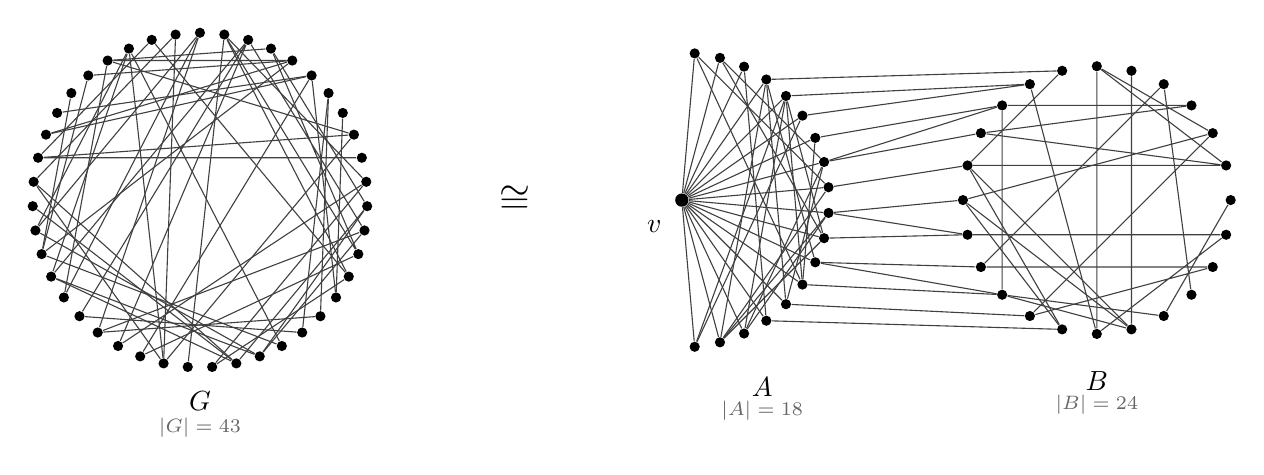
\begin{tikzpicture}[scale=0.85,
			vertex/.style={circle, fill, inner sep=1.3pt},
			pivot/.style={circle, fill, inner sep=1.7pt},
			e/.style={thin, black!75}
		]
		% Pivot vertex.
		\node[pivot, label={[label distance=1mm]below left:$v$}] (v) at (0,0) {};

		% Neighborhood A: 18 vertices, all adjacent to v.
		\foreach \i in {0,...,17} {
				\node[vertex] (a\i) at ({-85 + 10*\i}:2.2) {};
			}

		% Anti-neighborhood B: 24 vertices, none adjacent to v.
		\foreach \i [evaluate=\i as \bx using 6.2 + 2*cos(15*\i),
			evaluate=\i as \by using 2*sin(15*\i)] in {0,...,23} {
				\node[vertex] (b\i) at (\bx, \by) {};
			}

		% The whole graph G: 43 vertices on a circle.
		\foreach \i [evaluate=\i as \gx using -7.2 + 2.5*cos(90 + 8.372093*\i),
			evaluate=\i as \gy using 2.5*sin(90 + 8.372093*\i)] in {0,...,42} {
				\node[vertex] (g\i) at (\gx, \gy) {};
			}

		% Illustrative random edges inside G.
		\draw[e] (g13) -- (g39) (g16) -- (g41) (g18) -- (g41);
		\draw[e] (g1) -- (g10) (g32) -- (g40) (g10) -- (g23);
		\draw[e] (g3) -- (g25) (g9) -- (g34) (g29) -- (g42);
		\draw[e] (g18) -- (g33) (g19) -- (g38) (g0) -- (g12);
		\draw[e] (g20) -- (g35) (g33) -- (g42) (g1) -- (g20);
		\draw[e] (g30) -- (g40) (g30) -- (g42) (g31) -- (g41);
		\draw[e] (g0) -- (g17) (g21) -- (g42) (g7) -- (g38);
		\draw[e] (g14) -- (g24) (g8) -- (g39) (g5) -- (g13);
		\draw[e] (g4) -- (g39) (g22) -- (g33) (g0) -- (g15);
		\draw[e] (g24) -- (g32) (g10) -- (g20) (g3) -- (g20);
		\draw[e] (g14) -- (g23) (g19) -- (g30) (g3) -- (g12);
		\draw[e] (g12) -- (g24) (g17) -- (g27) (g28) -- (g38);
		\draw[e] (g17) -- (g31) (g4) -- (g40) (g3) -- (g14);
		\draw[e] (g13) -- (g25) (g4) -- (g15) (g9) -- (g35);
		\draw[e] (g8) -- (g38) (g23) -- (g32) (g24) -- (g31);
		\draw[e] (g5) -- (g39) (g6) -- (g13) (g27) -- (g37);
		\draw[e] (g22) -- (g29) (g14) -- (g41) (g11) -- (g23);
		\draw[e] (g16) -- (g26) (g2) -- (g29) (g2) -- (g9);
		\draw[e] (g28) -- (g36) (g26) -- (g37) (g4) -- (g35);

		% Edges from v into A.
		\foreach \i in {0,...,17} \draw[e] (v) -- (a\i);

		% Illustrative edges inside A.
		\draw[e] (a4) -- (a14) (a2) -- (a8) (a1) -- (a9);
		\draw[e] (a1) -- (a7) (a2) -- (a13) (a5) -- (a11);
		\draw[e] (a0) -- (a12) (a1) -- (a8) (a4) -- (a10);
		\draw[e] (a1) -- (a14) (a6) -- (a14) (a3) -- (a15);
		\draw[e] (a5) -- (a13) (a2) -- (a10) (a9) -- (a17);
		\draw[e] (a5) -- (a17) (a10) -- (a16) (a7) -- (a16);
		\draw[e] (a0) -- (a13) (a7) -- (a13);

		% Illustrative edges inside B.
		\draw[e] (b6) -- (b18) (b4) -- (b14) (b12) -- (b19);
		\draw[e] (b13) -- (b23) (b15) -- (b19) (b5) -- (b19);
		\draw[e] (b0) -- (b20) (b18) -- (b23) (b16) -- (b22);
		\draw[e] (b1) -- (b6) (b15) -- (b20) (b3) -- (b9);
		\draw[e] (b11) -- (b19) (b1) -- (b11) (b1) -- (b10);
		\draw[e] (b2) -- (b6) (b11) -- (b17) (b3) -- (b10);
		\draw[e] (b2) -- (b12) (b2) -- (b16) (b4) -- (b21);
		\draw[e] (b7) -- (b11) (b8) -- (b18) (b9) -- (b15);
		\draw[e] (b12) -- (b17) (b14) -- (b22);

		% Illustrative cross edges between A and B.
		\draw[e] (a8) -- (b12) (a9) -- (b11) (a7) -- (b13)
		(a10) -- (b10) (a6) -- (b14) (a11) -- (b9) (a5) -- (b15);
		\draw[e] (a3) -- (b17) (a4) -- (b16) (a6) -- (b15)
		(a8) -- (b13) (a10) -- (b9) (a12) -- (b8)
		(a13) -- (b8) (a14) -- (b7);

		% Isomorphism between the two depictions.
		\node[font=\Large] at (-2.5, 0) {$\cong$};

		% Group labels.
		\node at (-7.2, -3.0) {$G$};
		\node[font=\scriptsize, text=black!60] at (-7.2, -3.4) {$|G| = 43$};
		\node at (1.2, -2.8) {$A$};
		\node[font=\scriptsize, text=black!60] at (1.2, -3.15) {$|A| = 18$};
		\node at (6.2, -2.7) {$B$};
		\node[font=\scriptsize, text=black!60] at (6.2, -3.05) {$|B| = 24$};
	\end{tikzpicture}
	\caption{Illustrative decomposition into pivot $v$, neighborhood $A$ and anti-neighborhood $B$.}
\end{figure}
.

\begin{figure}[ht]
	\centering
	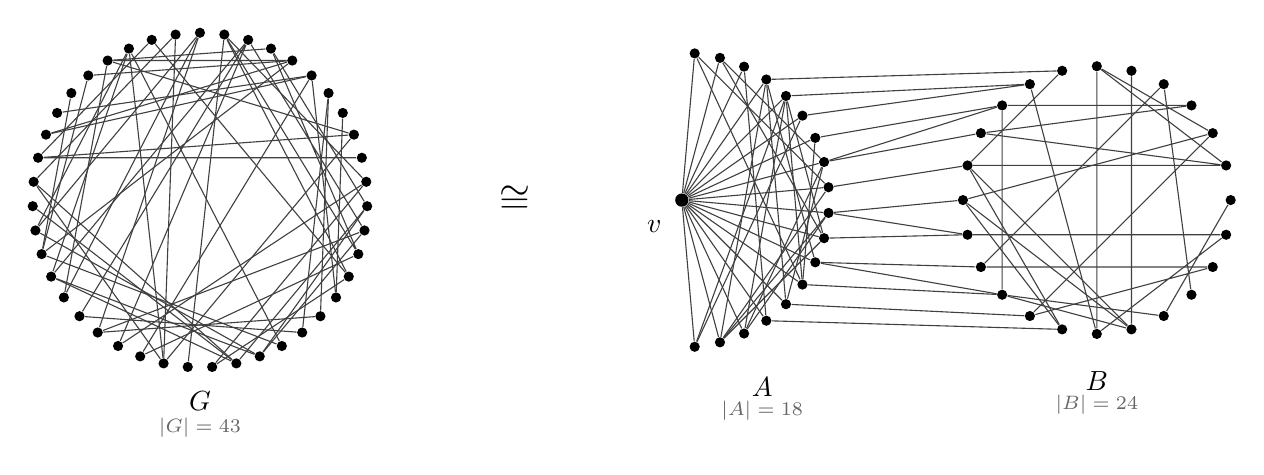
\begin{tikzpicture}[scale=0.85,
			vertex/.style={circle, fill, inner sep=1.3pt},
			pivot/.style={circle, fill, inner sep=1.7pt},
			e/.style={thin, black!75}
		]
		% Pivot vertex.
		\node[pivot, label={[label distance=1mm]below left:$v$}] (v) at (0,0) {};

		% Neighborhood A: 18 vertices, all adjacent to v.
		\foreach \i in {0,...,17} {
				\node[vertex] (a\i) at ({-85 + 10*\i}:2.2) {};
			}

		% Anti-neighborhood B: 24 vertices, none adjacent to v.
		\foreach \i [evaluate=\i as \bx using 6.2 + 2*cos(15*\i),
			evaluate=\i as \by using 2*sin(15*\i)] in {0,...,23} {
				\node[vertex] (b\i) at (\bx, \by) {};
			}

		% The whole graph G: 43 vertices on a circle.
		\foreach \i [evaluate=\i as \gx using -7.2 + 2.5*cos(90 + 8.372093*\i),
			evaluate=\i as \gy using 2.5*sin(90 + 8.372093*\i)] in {0,...,42} {
				\node[vertex] (g\i) at (\gx, \gy) {};
			}

		% Illustrative random edges inside G.
		\draw[e] (g13) -- (g39) (g16) -- (g41) (g18) -- (g41);
		\draw[e] (g1) -- (g10) (g32) -- (g40) (g10) -- (g23);
		\draw[e] (g3) -- (g25) (g9) -- (g34) (g29) -- (g42);
		\draw[e] (g18) -- (g33) (g19) -- (g38) (g0) -- (g12);
		\draw[e] (g20) -- (g35) (g33) -- (g42) (g1) -- (g20);
		\draw[e] (g30) -- (g40) (g30) -- (g42) (g31) -- (g41);
		\draw[e] (g0) -- (g17) (g21) -- (g42) (g7) -- (g38);
		\draw[e] (g14) -- (g24) (g8) -- (g39) (g5) -- (g13);
		\draw[e] (g4) -- (g39) (g22) -- (g33) (g0) -- (g15);
		\draw[e] (g24) -- (g32) (g10) -- (g20) (g3) -- (g20);
		\draw[e] (g14) -- (g23) (g19) -- (g30) (g3) -- (g12);
		\draw[e] (g12) -- (g24) (g17) -- (g27) (g28) -- (g38);
		\draw[e] (g17) -- (g31) (g4) -- (g40) (g3) -- (g14);
		\draw[e] (g13) -- (g25) (g4) -- (g15) (g9) -- (g35);
		\draw[e] (g8) -- (g38) (g23) -- (g32) (g24) -- (g31);
		\draw[e] (g5) -- (g39) (g6) -- (g13) (g27) -- (g37);
		\draw[e] (g22) -- (g29) (g14) -- (g41) (g11) -- (g23);
		\draw[e] (g16) -- (g26) (g2) -- (g29) (g2) -- (g9);
		\draw[e] (g28) -- (g36) (g26) -- (g37) (g4) -- (g35);

		% Edges from v into A.
		\foreach \i in {0,...,17} \draw[e] (v) -- (a\i);

		% Illustrative edges inside A.
		\draw[e] (a4) -- (a14) (a2) -- (a8) (a1) -- (a9);
		\draw[e] (a1) -- (a7) (a2) -- (a13) (a5) -- (a11);
		\draw[e] (a0) -- (a12) (a1) -- (a8) (a4) -- (a10);
		\draw[e] (a1) -- (a14) (a6) -- (a14) (a3) -- (a15);
		\draw[e] (a5) -- (a13) (a2) -- (a10) (a9) -- (a17);
		\draw[e] (a5) -- (a17) (a10) -- (a16) (a7) -- (a16);
		\draw[e] (a0) -- (a13) (a7) -- (a13);

		% Illustrative edges inside B.
		\draw[e] (b6) -- (b18) (b4) -- (b14) (b12) -- (b19);
		\draw[e] (b13) -- (b23) (b15) -- (b19) (b5) -- (b19);
		\draw[e] (b0) -- (b20) (b18) -- (b23) (b16) -- (b22);
		\draw[e] (b1) -- (b6) (b15) -- (b20) (b3) -- (b9);
		\draw[e] (b11) -- (b19) (b1) -- (b11) (b1) -- (b10);
		\draw[e] (b2) -- (b6) (b11) -- (b17) (b3) -- (b10);
		\draw[e] (b2) -- (b12) (b2) -- (b16) (b4) -- (b21);
		\draw[e] (b7) -- (b11) (b8) -- (b18) (b9) -- (b15);
		\draw[e] (b12) -- (b17) (b14) -- (b22);

		% Illustrative cross edges between A and B.
		\draw[e] (a8) -- (b12) (a9) -- (b11) (a7) -- (b13)
		(a10) -- (b10) (a6) -- (b14) (a11) -- (b9) (a5) -- (b15);
		\draw[e] (a3) -- (b17) (a4) -- (b16) (a6) -- (b15)
		(a8) -- (b13) (a10) -- (b9) (a12) -- (b8)
		(a13) -- (b8) (a14) -- (b7);

		% Isomorphism between the two depictions.
		\node[font=\Large] at (-2.5, 0) {$\cong$};

		% Group labels.
		\node at (-7.2, -3.0) {$G$};
		\node[font=\scriptsize, text=black!60] at (-7.2, -3.4) {$|G| = 43$};
		\node at (1.2, -2.8) {$A$};
		\node[font=\scriptsize, text=black!60] at (1.2, -3.15) {$|A| = 18$};
		\node at (6.2, -2.7) {$B$};
		\node[font=\scriptsize, text=black!60] at (6.2, -3.05) {$|B| = 24$};
	\end{tikzpicture}
	\caption{Illustrative decomposition into pivot $v$, neighborhood $A$ and anti-neighborhood $B$.}
\end{figure}
.

\begin{figure}[ht]
	\centering
	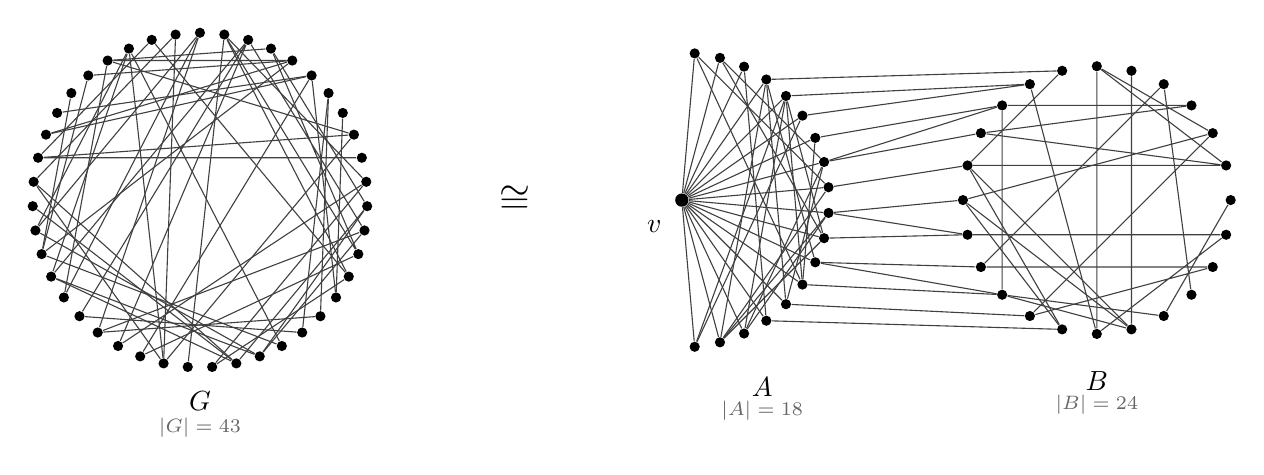
\begin{tikzpicture}[scale=0.85,
			vertex/.style={circle, fill, inner sep=1.3pt},
			pivot/.style={circle, fill, inner sep=1.7pt},
			e/.style={thin, black!75}
		]
		% Pivot vertex.
		\node[pivot, label={[label distance=1mm]below left:$v$}] (v) at (0,0) {};

		% Neighborhood A: 18 vertices, all adjacent to v.
		\foreach \i in {0,...,17} {
				\node[vertex] (a\i) at ({-85 + 10*\i}:2.2) {};
			}

		% Anti-neighborhood B: 24 vertices, none adjacent to v.
		\foreach \i [evaluate=\i as \bx using 6.2 + 2*cos(15*\i),
			evaluate=\i as \by using 2*sin(15*\i)] in {0,...,23} {
				\node[vertex] (b\i) at (\bx, \by) {};
			}

		% The whole graph G: 43 vertices on a circle.
		\foreach \i [evaluate=\i as \gx using -7.2 + 2.5*cos(90 + 8.372093*\i),
			evaluate=\i as \gy using 2.5*sin(90 + 8.372093*\i)] in {0,...,42} {
				\node[vertex] (g\i) at (\gx, \gy) {};
			}

		% Illustrative random edges inside G.
		\draw[e] (g13) -- (g39) (g16) -- (g41) (g18) -- (g41);
		\draw[e] (g1) -- (g10) (g32) -- (g40) (g10) -- (g23);
		\draw[e] (g3) -- (g25) (g9) -- (g34) (g29) -- (g42);
		\draw[e] (g18) -- (g33) (g19) -- (g38) (g0) -- (g12);
		\draw[e] (g20) -- (g35) (g33) -- (g42) (g1) -- (g20);
		\draw[e] (g30) -- (g40) (g30) -- (g42) (g31) -- (g41);
		\draw[e] (g0) -- (g17) (g21) -- (g42) (g7) -- (g38);
		\draw[e] (g14) -- (g24) (g8) -- (g39) (g5) -- (g13);
		\draw[e] (g4) -- (g39) (g22) -- (g33) (g0) -- (g15);
		\draw[e] (g24) -- (g32) (g10) -- (g20) (g3) -- (g20);
		\draw[e] (g14) -- (g23) (g19) -- (g30) (g3) -- (g12);
		\draw[e] (g12) -- (g24) (g17) -- (g27) (g28) -- (g38);
		\draw[e] (g17) -- (g31) (g4) -- (g40) (g3) -- (g14);
		\draw[e] (g13) -- (g25) (g4) -- (g15) (g9) -- (g35);
		\draw[e] (g8) -- (g38) (g23) -- (g32) (g24) -- (g31);
		\draw[e] (g5) -- (g39) (g6) -- (g13) (g27) -- (g37);
		\draw[e] (g22) -- (g29) (g14) -- (g41) (g11) -- (g23);
		\draw[e] (g16) -- (g26) (g2) -- (g29) (g2) -- (g9);
		\draw[e] (g28) -- (g36) (g26) -- (g37) (g4) -- (g35);

		% Edges from v into A.
		\foreach \i in {0,...,17} \draw[e] (v) -- (a\i);

		% Illustrative edges inside A.
		\draw[e] (a4) -- (a14) (a2) -- (a8) (a1) -- (a9);
		\draw[e] (a1) -- (a7) (a2) -- (a13) (a5) -- (a11);
		\draw[e] (a0) -- (a12) (a1) -- (a8) (a4) -- (a10);
		\draw[e] (a1) -- (a14) (a6) -- (a14) (a3) -- (a15);
		\draw[e] (a5) -- (a13) (a2) -- (a10) (a9) -- (a17);
		\draw[e] (a5) -- (a17) (a10) -- (a16) (a7) -- (a16);
		\draw[e] (a0) -- (a13) (a7) -- (a13);

		% Illustrative edges inside B.
		\draw[e] (b6) -- (b18) (b4) -- (b14) (b12) -- (b19);
		\draw[e] (b13) -- (b23) (b15) -- (b19) (b5) -- (b19);
		\draw[e] (b0) -- (b20) (b18) -- (b23) (b16) -- (b22);
		\draw[e] (b1) -- (b6) (b15) -- (b20) (b3) -- (b9);
		\draw[e] (b11) -- (b19) (b1) -- (b11) (b1) -- (b10);
		\draw[e] (b2) -- (b6) (b11) -- (b17) (b3) -- (b10);
		\draw[e] (b2) -- (b12) (b2) -- (b16) (b4) -- (b21);
		\draw[e] (b7) -- (b11) (b8) -- (b18) (b9) -- (b15);
		\draw[e] (b12) -- (b17) (b14) -- (b22);

		% Illustrative cross edges between A and B.
		\draw[e] (a8) -- (b12) (a9) -- (b11) (a7) -- (b13)
		(a10) -- (b10) (a6) -- (b14) (a11) -- (b9) (a5) -- (b15);
		\draw[e] (a3) -- (b17) (a4) -- (b16) (a6) -- (b15)
		(a8) -- (b13) (a10) -- (b9) (a12) -- (b8)
		(a13) -- (b8) (a14) -- (b7);

		% Isomorphism between the two depictions.
		\node[font=\Large] at (-2.5, 0) {$\cong$};

		% Group labels.
		\node at (-7.2, -3.0) {$G$};
		\node[font=\scriptsize, text=black!60] at (-7.2, -3.4) {$|G| = 43$};
		\node at (1.2, -2.8) {$A$};
		\node[font=\scriptsize, text=black!60] at (1.2, -3.15) {$|A| = 18$};
		\node at (6.2, -2.7) {$B$};
		\node[font=\scriptsize, text=black!60] at (6.2, -3.05) {$|B| = 24$};
	\end{tikzpicture}
	\caption{Illustrative decomposition into pivot $v$, neighborhood $A$ and anti-neighborhood $B$.}
\end{figure}


\begin{lemma}\label{R_5_5_43_degree_mem}
	Let $G \in R(5,5,43)$ be a Ramsey graph,
	then $18 \leqslant d(v) \leqslant 24$ for any vertex $v \in V(G)$.
\end{lemma}
\begin{proof}
	Pick an arbitrary vertex $v \in V(G)$.
	\begin{itemize}
		\item $G[N(v)]$ is $(4, 5)$-free, since any $K_4$ in $G[N(v)]$ can be extended with $v$ to a $K_5$ in $G$.
		\item $G[M(v)]$ is $(5, 4)$-free, since any $I_4$ in $G[M(v)]$ can be extended with $v$ to a $I_5$ in $G$.
	\end{itemize}
	Recall that $R(4, 5) = R(5, 4) = 25$.
	\begin{itemize}
		\item The neighborhood of $v$ therefor must have less than $25$ vertices.
		\item By complement symmetry, the anti-neighborhood of $v$ is larger than $43 - 1 - 25 = 17$ vertices.
	\end{itemize}
	It follows that for an arbitrary vertex $v$ the degree is bounded with $18 \leqslant d(v) \leqslant 24$
\end{proof}

\begin{theorem}[Even Pivot Theorem]
	Let $G \in R(5,5,43)$ be a ramsey graph up to complement.
	Then there exists a vertex $v \in V(G)$ with $d(v) = 18$ or $d(v) = 20$.
\end{theorem}
\begin{proof}
	The handshake lemma guarantees an even degree vertex in a graph of odd order.
	Combined with lemma \ref{R_5_5_43_degree_mem} we get four cases:
	\begin{itemize}
		\item $d(v) = 18$ or $d(v) = 20$: done.
		\item $d(v) = 22$ or $d(v) = 24$: The complement $G^c$ is still a Ramsey graph.
		      From counting all neighbors $d_G(v)$, all non-neighbors $d_{G^c}(v)$ and $v$ itself,
		      we get that $d_G(v) + d_{G^c}(v) + 1 = 43$.
		      Hence, in the complement graph, $v$ has either $18$ or $20$ neighboring vertices.
	\end{itemize}
\end{proof}

Now we can split the problem into two subproblems, one for each pivot degree.
We can further split the problem by the number of \emph{cross edges} $x = |e(A, B)|$
with one end-point in $A$ and the other in $B$.
$$e(A, B) = \left\{ \{u,w\} \in E(G) \mid u \in A, w \in B \right\}$$

We formalize this as a cross adjacency matrix $M$ over $\{ 0, 1\}$ with shapes $18 \times 24$ or $20 \times 22$.

$$M_{uw} = 1 \iff \{ u, w\} \in e(A, B)$$

Let $u \in A$, the row $u$ in this matrix corresponds to $R_u = N_B(u) \subseteq B$,
and a column $w \in B$ to $C_w = N_A(w) \subseteq A$.
This decomposes our problem into choosing a pivot $v$, then finding its induced (anti-)neighborhood $G[A], G[B]$ and finally the cross interface $M$.

\section{Neighborhood Connectivity}

Perhaps not the first question, but a fruitful one to ask is whether $G[A]$ is connected.
The answer is no, but the obstructions can be made explicit and lead to a complete partitioning of the degree-18 branch.
For most configurations $G[A]$ is connected, and otherwise,
we can show that it splits into a clique and a smaller connected Ramsey graph.

\begin{theorem}
	Let $G \in R(5, 5, 43)$ and $v \in V(G)$ with $d_G(v) = 18$.
	Then $G[N(v)]$ is either connected or $K_m \sqcup R$ for $m \in \{1, 2, 3\}$,
	where $K_m$ is a clique and $R \in R(4,4,18-m)$ is the connected residual graph.
\end{theorem}
\begin{proof}
	Let $A = N(v)$ which induces $G[A] \in R(4, 5, 18)$.
	By lemma \ref{A-has-I4} we know that $\alpha(A) = 4$.
	If $G[A]$ is connected we are done, so assume that $G[A]$ is disconnected.
	Pick an arbitrary component $S \subsetneq A$. Observe that both $S, S^c$ are non-empty and have no cross edges.
	The independence number behaves additive $\alpha(S) + \alpha(S^c) = \alpha(G[A]) = 4$ for anticonnected cuts.

	We show that one of the two components has to be a clique by deriving a contradiction.
	Assume for this purpose that $S, S^c$ are not a clique and therefor contain an independent pair.
	It follows that $S^c$ is $I_3$-free because an $I_3 \in S^c$ with the $I_2 \in S$ would extend to a forbidden $I_5 \in G$.
	The argument holds symmetrically for $S$.
	Note that $\alpha(S) + \alpha(S^c) = 2 + 2 = 4 = \alpha(G[A])$,
	hence there cannot be another component under the current assumptions.
	However, $R(4, 3) = 9$ which means $\abs{S}, \abs{S^c} < 9$.
	It follows that $\abs{S} + \abs{S^c} < 16 < 18 = \abs{A}$. contradiction.

	We have established that $G[A] = K_m \sqcup R$ and since $G[A]$ is $K_4$-free, $m \leqslant 3$.
	It remains to be shown that $R$ is connected and $(4,4)$-free.
\end{proof}

\section{Anchor Method}

Suppose $G \in R(5, 5, 43)$ with $A = N(v)$ and $B = M(v)$ for some degree-18 pivot $v \in V(G)$.

\begin{lemma}[Anchor Existence Lemma]\label{A-has-I4}
	$G[A]$ contains an independent 4-set $I_4 \subset A$.
\end{lemma}
\begin{proof}
	Recall that $R(4, 4) = 18$ and $|A| = 18$.
	It follows that $G[A]$ must contain a $K_4$ or an $I_4$.
	However, any $K_4$ could be extended with $v$ to form an $K_5$
	which contradicts the assumption $G \in R(5, 5, 43)$.
\end{proof}

Now that we have established that every $A$ contains an independent $4$-set,
we can use this as \emph{anchor}.
There might be multiple independent $4$-sets in $A$ so we pick the one with the largest min-degree.

% TODO: repeat the min-degree figure from below but with W_A replaced by \sum_A d(v)
% and q replaced by e(G[A]) and the axis values adapted accordingly.

\section{Cross Edge Counts}

The next split we perform in the search tree is by cross edge count $x = |e(A, B)|$.
We know $136 \leqslant x \leqslant 279$.
Many of our theorems are conditioned on the edge deficiency and degree excess:

\begin{definition}[Edge Deficiency]
	The \emph{edge deficiency} $q = 85 - e(A) \geqslant 0$ measures how sparse $G[A]$ is,
	by counting how many edges are missing from the extremal $E(4, 5, 18) \leqslant 85$ bound.
\end{definition}

\begin{definition}[Degree Excess]
	The \emph{total degree excess} $W_A = \sum_{u \in A} \left( d_G(u) - 18 \right)$ counts
	for all vertices in $A$ how far above the lower bound $d_G(u) \leqslant 18$ their degrees are.
\end{definition}

These two notions are tightly connected as can be shown with the handshake lemma.

\begin{lemma}[Cross Identity]
	$x - 136 = 2q + W_A$
\end{lemma}

\begin{center}
	\begin{tabular}{c|c|c}
		$x$          & cell            & notes \\
		\hline
		$136$        & $q=0$           &       \\
		$[137, 141]$ & $q \leqslant 2$ &       \\
		$[142, 143]$ & $q \leqslant 3$ &       \\
		$[144, 155]$ &                 &       \\
		$[156, 167]$ &                 &       \\
		$[168, 279]$ &                 &       \\
	\end{tabular}
\end{center}

% Data: research/n43/d18/parameter_landscape.json (schema version 1).
% Frontier window only: 0 <= q <= 17, 0 <= E_A = W_A <= 35.
% Inclusive JSON ranges become rectangles covering their integer cells.
\begin{figure}[htbp]
	\centering
	\begingroup
	\definecolor{landscape0}{HTML}{F7FBFF}
	\definecolor{landscape1}{HTML}{DEEBF7}
	\definecolor{landscape2}{HTML}{C6DBEF}
	\definecolor{landscape3}{HTML}{9ECAE1}
	\definecolor{landscape4}{HTML}{6BAED6}
	\definecolor{landscape5}{HTML}{4292C6}
	\definecolor{landscape6}{HTML}{2171B5}
	\definecolor{landscape7}{HTML}{08519C}
	\definecolor{landscape8}{HTML}{08306B}
	\begin{minipage}[t]{0.49\linewidth}
		\centering
		\textbf{(a) min-degree of forced $I_4 \subset A$}\par\smallskip
		\begin{tikzpicture}[x=0.28cm, y=0.115cm, font=\scriptsize]
			% Entries are q / first excess / last excess / lower bound.
			\foreach \q/\lo/\hi/\value in {
					0/0/1/8,
					0/2/9/7,
					0/10/15/6,
					0/16/19/5,
					0/20/23/4,
					0/24/34/3,
					0/35/35/2,
					1/0/0/8,
					1/1/8/7,
					1/9/13/6,
					1/14/17/5,
					1/18/21/4,
					1/22/29/3,
					1/30/35/2,
					2/0/7/7,
					2/8/12/6,
					2/13/16/5,
					2/17/20/4,
					2/21/28/3,
					2/29/35/2,
					3/0/6/7,
					3/7/11/6,
					3/12/15/5,
					3/16/19/4,
					3/20/23/3,
					3/24/35/2,
					4/0/5/7,
					4/6/10/6,
					4/11/14/5,
					4/15/17/4,
					4/18/22/3,
					4/23/35/2,
					5/0/4/7,
					5/5/9/6,
					5/10/12/5,
					5/13/15/4,
					5/16/21/3,
					5/22/35/2,
					6/0/3/7,
					6/4/8/6,
					6/9/11/5,
					6/12/14/4,
					6/15/17/3,
					6/18/29/2,
					6/30/35/1,
					7/0/2/7,
					7/3/7/6,
					7/8/10/5,
					7/11/13/4,
					7/14/16/3,
					7/17/23/2,
					7/24/35/1,
					8/0/1/7,
					8/2/6/6,
					8/7/9/5,
					8/10/11/4,
					8/12/15/3,
					8/16/22/2,
					8/23/35/1,
					9/0/0/7,
					9/1/2/6,
					9/3/3/5,
					9/4/4/4,
					9/5/5/3,
					9/6/17/2,
					9/18/35/1,
					10/0/1/6,
					10/2/2/5,
					10/3/3/4,
					10/4/4/3,
					10/5/5/2,
					10/6/35/1,
					11/0/0/6,
					11/1/1/5,
					11/2/2/4,
					11/3/3/3,
					11/4/4/2,
					11/5/5/1,
					11/6/35/0,
					12/0/0/5,
					12/1/1/4,
					12/2/2/3,
					12/3/3/2,
					12/4/4/1,
					12/5/35/0,
					13/0/0/4,
					13/1/1/3,
					13/2/2/2,
					13/3/3/1,
					13/4/35/0,
					14/0/0/3,
					14/1/1/2,
					14/2/2/1,
					14/3/35/0,
					15/0/0/2,
					15/1/1/1,
					15/2/35/0,
					16/0/0/1,
					16/1/35/0,
					17/0/35/0
				} {
					\pgfmathtruncatemacro{\shade}{\value}
					\fill[fill=landscape\shade] (\q,\lo) rectangle ({\q+1},{\hi+1});
				}
			\foreach \q in {1,...,17}
			\draw[white, opacity=0.35, very thin] (\q,0) -- (\q,36);
			% Cell centers are (q+0.5,W_A+0.5), so 2X+Y = (x-136)+1.5.
			\foreach \level in {10,20,...,60} {
					\pgfmathsetmacro{\leftq}{max(0,(\level-34.5)/2)}
					\pgfmathsetmacro{\rightq}{min(18,(\level+1.5)/2)}
					\draw[red!75!black, dashed, thin]
					(\leftq,{\level+1.5-2*\leftq}) --
					(\rightq,{\level+1.5-2*\rightq})
					node[midway, fill=white, inner sep=1pt] {$\level$};
				}
			\draw[black!50, thin] (0,0) rectangle (18,36);
			\foreach \q in {0,3,6,9,12,15,17} {
					\draw[black!50] ({\q+0.5},0) -- ++(0,-0.7);
					\node[below, inner sep=2pt] at ({\q+0.5},-0.7) {$\q$};
				}
			\foreach \excess in {0,5,10,15,20,25,30,35} {
					\draw[black!50] (0,{\excess+0.5}) -- ++(-0.25,0);
					\node[left, inner sep=2pt] at (-0.25,{\excess+0.5}) {$\excess$};
				}
			\node[below] at (9,-3.6) {$q$};
			\node[rotate=90] at (-2.7,18) {$W_A$};
		\end{tikzpicture}\par\smallskip
		\begin{tikzpicture}[x=0.47cm, y=0.3cm, font=\scriptsize]
			\foreach \value in {0,1,2,3,4,5,6,7,8} {
					\fill[fill=landscape\value] (\value,0) rectangle ++(1,1);
					\node[below, inner sep=2pt] at ({\value+0.5},0) {$\value$};
				}
			\draw[black!40, thin] (0,0) rectangle (9,1);
		\end{tikzpicture}
	\end{minipage}
	\hfill
	\begin{minipage}[t]{0.49\linewidth}
		\centering
		\textbf{(b) Minimum column size}\par\smallskip
		\begin{tikzpicture}[x=0.28cm, y=0.115cm, font=\scriptsize]
			% Entries are q / first excess / last excess / lower bound.
			\foreach \q/\lo/\hi/\value in {
					0/0/1/5,
					0/2/35/4,
					1/0/35/4,
					2/0/35/4,
					3/0/13/4,
					3/14/35/3,
					4/0/35/3,
					5/0/35/3,
					6/0/35/3,
					7/0/35/3,
					8/0/35/2,
					9/0/35/1,
					10/0/35/1,
					11/0/35/1,
					12/0/35/1,
					13/0/35/1,
					14/0/35/1,
					15/0/35/1,
					16/0/35/1,
					17/0/35/1
				} {
					\pgfmathtruncatemacro{\shade}{\value}
					\fill[fill=landscape\shade] (\q,\lo) rectangle ({\q+1},{\hi+1});
				}
			\foreach \q in {1,...,17}
			\draw[white, opacity=0.35, very thin] (\q,0) -- (\q,36);
			% Cell centers are (q+0.5,W_A+0.5), so 2X+Y = (x-136)+1.5.
			\foreach \level in {10,20,...,60} {
					\pgfmathsetmacro{\leftq}{max(0,(\level-34.5)/2)}
					\pgfmathsetmacro{\rightq}{min(18,(\level+1.5)/2)}
					\draw[red!75!black, dashed, thin]
					(\leftq,{\level+1.5-2*\leftq}) --
					(\rightq,{\level+1.5-2*\rightq})
					node[midway, fill=white, inner sep=1pt] {$\level$};
				}
			\draw[black!50, thin] (0,0) rectangle (18,36);
			\foreach \q in {0,3,6,9,12,15,17} {
					\draw[black!50] ({\q+0.5},0) -- ++(0,-0.7);
					\node[below, inner sep=2pt] at ({\q+0.5},-0.7) {$\q$};
				}
			\foreach \excess in {0,5,10,15,20,25,30,35} {
					\draw[black!50] (0,{\excess+0.5}) -- ++(-0.25,0);
					\node[left, inner sep=2pt] at (-0.25,{\excess+0.5}) {$\excess$};
				}
			\node[below] at (9,-3.6) {$q$};
			\node[rotate=90] at (-2.7,18) {$W_A$};
		\end{tikzpicture}\par\smallskip
		\begin{tikzpicture}[x=0.47cm, y=0.3cm, font=\scriptsize]
			\foreach \value in {0,1,2,3,4,5} {
					\fill[fill=landscape\value] (\value,0) rectangle ++(1,1);
					\node[below, inner sep=2pt] at ({\value+0.5},0) {$\value$};
				}
			\draw[black!40, thin] (0,0) rectangle (6,1);
		\end{tikzpicture}
	\end{minipage}
	\endgroup
	\caption{Each cell represents one integer pair $(q,W_A)$.
		In (a), the color corresponds to the interior min-degree of a forced independent set $I_4 \subseteq A$.
		The color zero indicates that no $I_4$ can be forced in $A$.
		In (b), the color $c$ guarantees $|C_w|\ge c$ for every $w\in B$.
		In both panels, dashed red contours are labeled by $x-136=2q+W_A$
		in increments of $10$, with integer parameter values located at cell centers.}
	\label{fig:parameter-landscape}
\end{figure}


\section{Cross Adjacency Conditions}

Suppose we have a hypothetical $G \in R(5, 5, 43)$ and we have pivoted on $v$ with $d_G(v) = 18$ which splits the graph into $A = N(v)$ and $B = M(v)$.
There are now several conditions we can impose based on the structure of the rows and columns of the cross adjacency matrix $M$.

\begin{theorem}[Cross Edge Bounds]
	$136 \leqslant \left| M \right| \leqslant 279$
\end{theorem}

\begin{theorem}[Neighborhood Edge Bounds]
	$50 \leqslant e(G[A]) \leqslant 85$
\end{theorem}

\begin{theorem}[Anti-Neighborhood Edge Bounds]
	$144 \leqslant e(G[B]) \leqslant 160$
\end{theorem}

\begin{theorem}[Neighborhood Degree Bounds]
	$0 \leqslant d_A(u) \leqslant 13$
\end{theorem}

\begin{theorem}[Anti-Neighborhood Degree Bounds]
	$10 \leqslant d_A(u) \leqslant 17$
\end{theorem}

\begin{theorem}[Row Multiplicity]
	No row repeats more than twice.
\end{theorem}

\begin{theorem}
	No row of size $9$ or $10$ repeats.
\end{theorem}

\section{Anti-Neighborhood Catalogue}

There is a complete catalogue of $R(5, 4, 24)$ consisting of $352366$ unique graphs up to isomorphism.
Therefor every potential $G[B]$ is already established and once we have picked a pivot and an anti-neighborhood $B$,
it remains to find (or exclude) any potential neighborhood $G[A]$ and cross adjacency matrix $M$.

The anti-neighborhood $G[B]$ is $K5$-free, $I5$-free and also $I4$-free, because otherwise it could be extended to an $I5$ in $G$.

\section{Transversals}

Let $\F = \{ F_i \}$ be a family of sets. A \emph{transversal} of $\F$ is a set $T$ such that $\forall S \in \F \colon S \cap T \neq \emptyset$

\section{AI Usage}

We dissect the galactic search space into multiple branches based on the degree of the pivot element.
For each branch we instruct LLMs (GPT-6.1 Sol and GLM-5.3) to derive analytical conditions to further split the search space.
We recurse until progress stalls, in which case we resort to SAT solvers to (cleverly) bruteforce the reduced search space.

This approach allows us to prune more families of graphs, since we have more specific theorems tailored to the subcase we are inspecting.

\section{Tools}

We use a \texttt{geng} from \texttt{nauty} (v2.9.3) to enumerate graphs.
Our fork of \texttt{geng} is customized to efficiently prune graphs with cliques or independent sets.

\section*{Glossary}

\begin{definition}[Edge Deficiency]
	Let $G \in R(s, t, n)$.
	The \emph{edge deficiency} $q = E(s, t, n) - |E(G)| \geqslant 0$ measures how sparse $G$ is
	with respect to the extremal edge bound $E(s, t, n)$.
\end{definition}

\begin{definition}[Degree Excess]
	Let $G$ be a simple graph.
	Assume $d_G(v) \geqslant k$ for all vertices $v \in V(G)$.
	Fix $v$, the \emph{degree excess} $\epsilon_v = d_G(v) - k$ is the difference between the degree of $v$ and the lower bound.
	Let $S \subseteq V(G)$, its \emph{total degree excess} is $$W_S = \sum_{v \in S} \epsilon_v = \sum_{v \in S} \left( d_G(v) - k \right)$$.
\end{definition}

\begin{definition}[Transversal]
	Let $\F = \{ F_i \}$ be a family of sets.
	A \emph{transversal} of $\F$ is a set $T$ such that $\forall S \in \F \colon S \cap T \neq \emptyset$.
	We write $\tau(\F)$ to denote the cardinality of the smallest transversal of $\F$.
\end{definition}

\nocite{angeltveit_mckay_2026,mckay_radziszowski_1992,
	biere_et_al_2024,elffers_nordstrom_2018,bolusani_et_al_2024,mckay_piperno_2014,de_moura_ullrich_2021}
\bibliographystyle{plain}
\bibliography{sources/angeltveit-mckay-2026,sources/mckay-radziszowski-1992,sources/tools}

\end{document}
